%\documentclass[handout, 11pt]{beamer} %For Handouts
\documentclass[11pt]{beamer}
\usetheme{Singapore}
\usefonttheme[header]{structuresmallcapsserif}
\usefonttheme{professionalfonts}

\usepackage{color,colortbl}
\usepackage{amssymb}
\usepackage{amsmath}
\usepackage{amsthm}
\usepackage{graphicx}
\usepackage{enumerate}
\usepackage{booktabs}
\usepackage{makecell}
\usepackage{multirow}
\usepackage{times}
\usepackage{float}
\usepackage{etoolbox}
\usepackage{dsfont}

\makeatletter
\patchcmd{\Ginclude@eps}{"#1"}{#1}{}{}
\makeatother
\usepackage{tikz}
\usetikzlibrary{positioning}
\usepackage{siunitx}
\sisetup{group-separator={,},group-four-digits=true}
\usepackage[labelformat=empty,scriptsize,singlelinecheck=off]{caption}
\captionsetup[subfigure]{font=scriptsize,labelfont=scriptsize}
\usepackage[font+=scriptsize]{subcaption}
\usepackage{xcolor}
\usepackage{comment}
\usepackage{tabularx}

\usepackage{accents}
\newcommand{\ubar}[1]{\underaccent{\bar}{#1}}
\newcommand{\overbar}[1]{\mkern 1.5mu\overline{\mkern-1.5mu#1\mkern-1.5mu}\mkern 1.5mu}
\setbeamertemplate{itemize subitem}[triangle]

% Set footline
\makeatletter
\setbeamertemplate{footline}
{%
\begin{beamercolorbox}[wd=\paperwidth,ht=0.5ex,dp=0ex,center]{footlinerule}
\end{beamercolorbox}%
\begin{beamercolorbox}[wd=\paperwidth,ht=0.6ex,dp=0ex,center]{empty}
\end{beamercolorbox}%
\leavevmode%
  \hbox{%
  \begin{beamercolorbox}[wd=\paperwidth,ht=2.25ex,dp=2ex,center]{author in head/foot}%
    \usebeamerfont{author in head/foot}%
    \insertshortauthor
  \end{beamercolorbox}}%
  \vskip0pt%
}
\makeatother

%Set Margins
\beamersetleftmargin{0.5cm}
\beamersetrightmargin{0.5cm}

%Imported File Type
\DeclareGraphicsExtensions{.eps}

%Remove Navigation Symbols
\setbeamertemplate{navigation symbols}{}

%Sets the transparency of uncovered text
\beamertemplatetransparentcoveredmedium

%Define New Font Sizes
\def\Tiny{\fontsize{5pt}{5pt}\selectfont}
\def\Scriptsize{\fontsize{8pt}{8pt}\selectfont}

%Table mid rule width
\newcommand{\otoprule}{\midrule[\heavyrulewidth]}

%Define Color Names
\definecolor{Gray}{rgb}{0.65,0.65,0.65}
\definecolor{darkblue}{rgb}{0,0,0.55}
\definecolor{darkred}{rgb}{0.5,0,0}
\definecolor{red}{rgb}{1,0,0}

% Counter for resuming enumeration across slides
\newcounter{savedenumi}

\newcommand{\scs}{\Tiny}

%%%%%%%%%%%%%%%%%%%%%%%%%%%%%%%%%%%%%%%%%%%%%%%%%%%%%%%%%%%%%%%%%%%%%%%%%%%%%%%%%%%%%%%%%%%%%%%%%%%%%%%%%%%%%%%%

    \title[]{Comparison of Global Solution Methods to a Zero Lower Bound Model}
    \author[]{\color{Gray} Emily Martell\thanks{\scriptsize{Thank you to Professor Throckmorton for advising and providing materials for this project. Thank you to Professor Campbell, Professor Han, Professor Rolek, and Professor Throckmorton for serving on my committee.}}}
    \date[]{College of William \& Mary \\ \today}


\begin{document}

%===============================================================================================================

{
\setbeamertemplate{footline}{}
    \frame{\titlepage}
}

%===============================================================================================================

\begin{frame}\frametitle{Introduction}

\begin{itemize}\setlength{\itemsep}{7pt}
  \item <1-|handout:1>As a result of the global financial crisis of 2007-9 and the subsequent recession, central banks lowered their policy rate to its zero lower bound (ZLB)
  \item  <2-|handout:1>The ZLB now holds for a significant portion of historic data for the US, Japan, and the Euro Area
  \item  <3-|handout:1>The ZLB introduces a kink in the central bank's policy rule and calls into question linear estimation methods
  \item <4-|handout:1> Responses in the literature to this nonlinearity include:
  %\item This paper:
  \begin{enumerate}\setlength{\itemsep}{4pt}
	\item  Failing to incorporate ZLB period data
	\item  Estimating linear models on the entire data set
	\item  Estimating a piecewise linear version of the nonlinear model (e.g., Guerrieri and Iacoviello, 2017)
	\item  Estimating fully nonlinear models that treats the ZLB as an occasionally binding constraint (e.g., Gust et al., 2017; Plante et al., 2018; Richter and Throckmorton, 2016).
  \end{enumerate}
\end{itemize}
\end{frame}

%=========================================================================
\begin{frame}\frametitle{The Model (With Capital)}
\begin{itemize}\setlength{\itemsep}{6pt}
\item <1-|handout:1>The households choose $\{c_t, n_t, b_t, x_t, k_t\}_{t=0}^\infty$ to maximize expected lifetime utility given by
\begin{gather*}
E_0\sum_{t=0}^\infty\beta[\log(c_t-hc^a_{t-1}) - \chi n_t^{1+\eta}/(1+\eta)],
\end{gather*} 
subject to their budget constraint
\begin{gather*}
    c_t+x_t+b_t/(i_ts_t)=w_tn_t+r_t^kk_{t-1}+b_{t-1}/\pi_t+d_t.
  \end{gather*} 
\item <2-|handout:1>The nominal bond, $b$, is subject to a risk premium, $s$, that follows
\begin{gather*}
  s_t = (1-\rho_s)\bar{s} + \rho_ss_{t-1} + \sigma_s\varepsilon_{s,t},
\end{gather*}
where $\bar{s}$ is the steady-state value. %An increase in $s_t$ boosts saving, which lowers period-$t$ demand.
\end{itemize}
\end{frame}
%=========================================================================
\begin{frame}\frametitle{Households}
\begin{itemize}\setlength{\itemsep}{8pt}
\item <1-|handout:1>Households also face an investment adjustment cost, so the law of motion for capital is given by
\begin{gather*}
  k_t = (1-\delta)k_{t-1} + x_t(1-\nu(x^g_t - 1)^2/2),\; 0 \leq \delta \leq 1.
  \end{gather*} %$x_t^g$ is investment growth relative to its steady-state and $\nu \geq 0$ scales the cost.
\item <2-|handout:1>The FOCs to the representative household's constrained optimization problem are
\scriptsize
\begin{gather*}
  \lambda_t = c_t - hc^a_{t-1}, \\
  w_t = \chi n_t^\eta \lambda_t,\\
  1 =  \beta E_t[(\lambda_t/\lambda_{t+1})(s_ti_t/(\bar{\pi}\pi_{t+1}^{gap}))],\\
  q_t = \beta E_t[(\lambda_t/\lambda_{t+1})(r^k_{t+1}+(1-\delta)q_{t+1})],\\
  1 = q_t[1-\nu(x^g_t-1)^2/2 - \nu(x_t^g-1)x_t^g] + \nu\beta\bar{g}E_t[q_{t+1}(\lambda_t/\lambda_{t+1})(x^g_{t+1})^2(x^g_{t+1}-1)].\\
\end{gather*} %where $1/\lambda$ is the marginal utility of consumption and $q$ is Tobin's q 
\normalsize
\end{itemize}
\end{frame}
%=========================================================================
\begin{frame}\frametitle{Firms}
\begin{itemize}\setlength{\itemsep}{8pt}
\item <1-|handout:1>The production sector consists of a continuum of monopolistically competitive intermediate goods firms and a final goods firm 
\item <2-|handout:1>Technology is $z_t = g_tz_{t-1}$, which is common across firms
\item <3-|handout:1>Deviations from the steady-state growth rate, $\bar{g}$, follow
\begin{gather*}
  g_t = \bar{g} + \sigma_g\varepsilon_{g,t}.
\end{gather*}
\item <4-|handout:1>In symmetric equilibrium, the optimality conditions reduce to
\scriptsize
\begin{gather*}
  y_t = (k_{t-1})^\alpha(z_tn_t)^{1-\alpha},\\
  w_t = (1-\alpha)mc_ty_t/n_t,\\
  r_t^k = \alpha mc_t y_t/k_{t-1},\\
  \varphi(\pi_t^{gap}-1)\pi_t^{gap} = 1-\theta + \theta mc_t + \beta\varphi E_t[(\lambda_t/\lambda_{t+1})(\pi_{t+1}^{gap}-1)\pi_{t+1}^{gap}(y_{t+1}/y_t)].
\end{gather*}
\normalfont
\end{itemize}
\end{frame}
%=========================================================================
\begin{frame}\frametitle{Monetary Policy}
\begin{itemize} \setlength{\itemsep}{14pt}
\item <1-|handout:1>\ 
The central bank sets the gross nominal interest rate, $i$, according to
\begin{gather*}
    i_t=\max\{1,i_t^n\},\\
  i_t^n=(i^n_{t-1})^{\rho_i}(\bar{\imath}(\pi^{gap}_t)^{\phi_\pi}(y^{g}_{t})^{\phi_y})^{1-\rho_i}\exp(\sigma_i\varepsilon_{i,t}). 
\end{gather*}
%where $y^{gdp}$ is real GDP (i.e., output, $y$, minus the resources lost due to adjustment costs, $adj^p$), $i^n$ is the gross notional interest rate, $\bar i$ and $\bar{\pi}$ are the target values of the inflation and nominal interest rates, and $\phi_\pi$ and $\phi_y$ are the responses to the inflation and output growth gaps. 
\item <2-|handout:1>A more negative net notional rate indicates that the central bank is more constrained
\end{itemize}
\end{frame}

%=========================================================================
\begin{frame}\frametitle{Competitive Equilibrium}\setlength{\itemindent}{-1.2em}
\begin{itemize} \setlength{\itemsep}{8pt}
\item <1-|handout:1>The aggregate resource constraint and real GDP definition are given by:
\begin{gather*}
  c_t + x_t = y_t^{gdp}\\
  y_t^{gdp} = [1 - \varphi(\pi_t^{gap}-1)^2/2]y_t
\end{gather*}
\item <2-|handout:1>The model does not have a steady-state due to the unit root in technology, $z_t$. Therefore, we define the variables with a trend in terms of technology (i.e., $\tilde{x}_t \equiv x_t/z_t$)
\end{itemize}
\end{frame}
%=========================================================================
\begin{frame}\frametitle{Competitive Equilibrium}
\begin{itemize} \setlength{\itemsep}{10pt}
\item <1-|handout:1>A competitive equilibrium consists of sequences of 
\begin{enumerate} \setlength{\itemsep}{5pt}
\item quantities, $\{\tilde{c}_t, \tilde{y}_t, \tilde{y}_t^{gdp}, x^g_t, y^g_t, n_t, \tilde{k}_t, \tilde{x}_t\}_{t=0}^\infty$ \item prices, $\{\tilde{w}_t, i_t, i^n_t, \pi_t, \tilde{\lambda}_t, q_t, r^k_t, mc_t\}_{t=0}^\infty$
\item exogenous variables, $\{s_t,g_t\}_{t=0}^\infty$
\end{enumerate}
\item <2-|handout:1>that satisfy the detrended equilibrium system, given 
\begin{enumerate}\setlength{\itemsep}{5pt}
\item the initial conditions, $\{\tilde{c}_{-1}, i^n_{-1}, \tilde{k}_{-1}, \tilde{x}_{-1}, \tilde{w}_{-1}, s_0, g_0, \varepsilon_{i,0}\}$
\item three sequences of shocks, $\{\varepsilon_{g,t}, \varepsilon_{s,t}, \varepsilon_{i,t}\}_{t=1}^\infty$
\end{enumerate}
\end{itemize}
\end{frame}
%===============================================================================================================
\begin{frame}\frametitle{Parameter Values}
\begin{table}[H]
\centering
\captionsetup{justification=centering}
  \scriptsize
    \setlength{\tabcolsep}{3pt}      
  \begin{tabular}{l c c |l  c c}
    \hline
  Subjective Discount Factor & $\beta$ & $0.9949$ & Rotemberg Price Adjustment Cost & $\varphi$ & $100$ \\
   Frisch Labor Supply Elasticity & $1/\eta$ & $3$ & Inflation Gap Response & $\phi_\pi$ & $2.0$ \\
  Price Elasticity of Substitution & $\theta$ & $6$ & Output Growth Gap Response & $\phi_y$ & $0.5$ \\
  Steady-State Labor Hours & $\bar{n}$ & $1/3$ & Habit Persistence & $h$ & $0.80$ \\
  Steady-State Risk Premium & $\bar{s}$ & $1.0058$ & Risk Premium Persistence & $\rho_s$ & $0.80$ \\
  Steady-State Growth Rate & $\bar{g}$ & $1.0034$ & Notional Rate Persistence & $\rho_i$ & $0.80$ \\
  Steady-State Inflation Rate & $\bar{\pi}$ & $1.0053$ & Technology Growth Shock SD & $\sigma_g$ & $0.005$ \\
  Capital Share of Income & $\alpha$ & $0.35$ & Risk Premium Shock SD & $\sigma_s$ & $0.0085$ \\
  Capital Depreciation Rate & $\delta$ & $0.025$ & Notional Interest Rate Shock SD & $\sigma_i$ & $0.002$ \\
  Investment Adjustment Cost & $\nu$ & $4$ & & &\\
  \hline
  \end{tabular}
\normalfont
\end{table}
\begin{itemize}\setlength{\itemsep}{8pt}
\item <2-|handout:1>Parameters are from Atkinson et al.\ (2019), and are chosen to be characteristic of U.S. data
\item <3-|handout:1>For the model without capital, $\sigma_s = 0.006$ %To allow the GHLS algorithm to converge
\end{itemize}
\end{frame}
%===============================================================================================================

\begin{frame}\frametitle{Nonlinear Solution Methods}
\begin{itemize}\setlength{\itemsep}{10pt}
	\item  <1-|handout:1>As it is important to incorporate all historic data and yield accurate parameter values and predictions, the path forward seems to be in fully nonlinear models
	\item <2-|handout:1>Solving nonlinear models with projection methods:
\begin{enumerate}
		\item  <3-|handout:1>Policy function iteration with linear interpolation on an evenly spaced grid (e.g., Plante et al., 2018; Richter and Throckmorton, 2016).
		\item  <3-|handout:1>Alternate approximating functions: regime-indexed policy functions (Gust et al., 2017), piecewise smooth policy functions (Aruoba et al. 2018)
		\item  <3-|handout:1>Alternate grid construction and policy function evaluation method: Smolyak method with Chebyshev polynomials (e.g., Gust et al., 2017; Ferna\'ndez-Villaverde et al. 2015; Aruoba et al., 2018)
	\end{enumerate}
\end{itemize}
\end{frame}

%=========================================================================
\begin{frame}\frametitle{Two Solution Methods}
\begin{table}\scriptsize
    \renewcommand*{\arraystretch}{1.4}
    \setlength{\tabcolsep}{6pt}      
  \begin{tabularx}{\textwidth}{l | X | X}
    \hline
    & \textbf{Atkinson et al.\ (2019)} & \textbf{Gust et al.\ (2017)} \\ \hline
    	Discretization Method & Evenly-spaced grid points & Smolyak Method\\
	Policy Function Evaluation & Linear Interpolation & Chebyshev Polynomials \\
	Integration Method & Rouwenhorst & Gauss-Hermite quadrature  \\ \hline
\end{tabularx}
\end{table}\normalsize
\begin{itemize}\setlength{\itemsep}{10pt}
\item  <2-|handout:1>Evenly-spaced grid points work well with linear interpolation
\item  <3-|handout:1>The Smolyak method is optimal for Chebyshev polynomials
\item  <4-|handout:1>The Rouwenhorst (1995) method improves approximation on exogenous dimensions when the driving processes are autoregressive
\end{itemize}

\end{frame}
%=========================================================================
\begin{frame}\frametitle{Atkinson et al.\ (2019)}
\begin{itemize}\setlength{\itemsep}{10pt}
\item <1-|handout:1> Time iteration with linear interpolation
\item <2-|handout:1>Directly approximates policy functions
\item <3-|handout:1> State space features evenly-spaced nodes
\item<4-|handout:1>  Exogenous variables are approximated with the Markov chain from Rouwenhorst (1995)
  \begin{itemize}\setlength{\itemsep}{4pt}
\item Only requires interpolation along the dimensions of the endogenous state variables
\end{itemize}
\end{itemize}
\end{frame}
%=========================================================================
\begin{frame}\frametitle{Gust et al.\ (2017)}
\begin{itemize}\setlength{\itemsep}{6pt}
\item  <1-|handout:1>Approximates policy functions using an anisotropic Smolyak method with Chebyshev polynomials
\item  <2-|handout:1>Approximates exogenous state variables using Gauss-Hermite quadrature%why if we know Rouwenhorst is better?
\item  <3-|handout:1>Instead of directly computing the policy functions, they estimate functions at and away from the ZLB, building on Christiano and Fisher (2000)
  \begin{itemize}\setlength{\itemsep}{4pt}
\item  Policy functions feature a kink or non-differentiability at the ZLB and regime-indexing the policy functions will yield smoother functions
\item Low-order Chebyshev polynomials perform better on smoother functions and are inexpensive to compute
\end{itemize}
\end{itemize}
\end{frame}
%=========================================================================
\begin{frame}\frametitle{This Project}
\begin{itemize}\setlength{\itemsep}{8pt}
\item  <1-|handout:1>In this project, we consider how splitting up the policy functions conditional on the ZLB impacts the speed and accuracy of the solution of a nonlinear model
\item  <2-|handout:1>We use policy function iteration on a fixed point with linear interpolation
\item  <3-|handout:1>Atkinson et al.\ (2019) directly computes the policy functions;  Gust et al.\ (2017) indirectly computes the policy functions through regime-indexed policy functions
\item <4-|handout:1> Solution algorithm based on Atkinson et al.\ (2019) denoted henceforth as ART; solution algorithm based on Gust et al.\ (2017) denoted henceforth as GHLS
\end{itemize}
\end{frame}
%=========================================================================
\begin{frame}\frametitle{Motivation for Regime-Indexed Policy Functions}
\begin{itemize}\setlength{\itemsep}{6pt}
\item  <1-|handout:1>The interest rate enters directly in the consumption Euler equation
\begin{gather*}
1 =  E_t[\beta(c_t/c_{t+1})(s_ti_t/\pi_t)],
\end{gather*}
where $E_t$ is the expectation operator, $0 < \beta < 1$ is the discount factor, and $c_t$, $s_t$, $i_t$, and $\pi_t$ are consumption, the risk premium, the interest rate, and inflation at time $t$. 
\begin{itemize} \small
\item $\beta(c_t/c_{t+1})$ is a stochastic discount factor used to value future real income
\item $s_ti_t/\pi_t$ is a real interest rate on a one-period bond
\end{itemize}\normalfont
\item <2-|handout:1> At the ZLB, the presence of the interest rate creates a nonlinearity in the consumption Euler equation 
\item <3-|handout:1> $c_t$ depends directly on the interest rate
\end{itemize}
\end{frame}%=========================================================================
\begin{frame}\frametitle{Our Solution Algorithm} %NEED TO PUT SOME ABOUT GHLS?
\begin{itemize}\setlength{\itemsep}{8pt}
\item   <1-|handout:1>Construct the state space with evenly-spaced nodes and approximate exogenous state variables with Rouwenhorst (1995)
\item  <2-|handout:1>Obtain initial conjectures for a set of policy functions from the log-linear solution
\item  <3-|handout:1>Using a fixed point iteration scheme, linearly interpolate and numerically integrate the policy functions each step
\begin{itemize}
\item For ART portion, we update a single policy function, and for the GHLS portion we update regime-indexed policy functions
\end{itemize}
\item <5-|handout:1> The algorithm converges once the maximum distance between successive guesses of policy functions falls below a convergence criterion

\end{itemize}
\end{frame}


%===================================================================================
\begin{frame}\frametitle{Discretized State Space (No Capital)}

\begin{itemize}\setlength{\itemsep}{10pt}
  \item <1-|handout:1>State variables: $g_t$, $s_t$, $mp_t$, $i^n_{t-1}$
  \item <2-|handout:1>Number of grid points: $N_g$, $N_{s}$, $N_{mp}$, $N_{i^n}$
  \item <3-|handout:1>Grid boundaries: 
\begin{center}
$[g_{\min},g_{\max}]$, $[s_{\min},s_{\max}]$, $[mp_{\min},mp_{\max}]$, $[i^n_{\min},i^n_{\max}]$
\end{center}
  \item <4-|handout:1>Create evenly spaced grids:
  \begin{center}
    $x_{grid} = \texttt{linspace}(x_{\min},x_{\max},N_x), \quad x\in\{g,s,mp,i^n\}$
  \end{center}
  \item <5-|handout:1>State space contains $N=N_g\times N_s\times N_{mp}\times N_{i^n}$ nodes
  \item <6-|handout:1>Create an array for each state variable, where every position is a unique permutation of the state space:
  \begin{center}
    $[g_{gr},s_{gr},mp_{gr},i^n_{gr}] = \texttt{ndgrid}(g_{grid},s_{grid},mp_{grid},i^n_{grid})$
  \end{center}
\end{itemize}

\end{frame}
%===================================================================================

\begin{frame}\frametitle{Functional Approximation}

\begin{itemize}\setlength{\itemsep}{12pt}
  \item <1-|handout:1>True RE solution only exists in special cases %(e.g., $\delta=1$)
  \item <2-|handout:1>Goal: Find an approximating function that maps the state space to the optimal decision rule for consumption:
  \begin{gather*}
    \underbrace{c(g,s,mp,i^n)}_{\textrm{True RE Solution}} \approx \underbrace{{\cal{P}}_c(g,s,mp,i^n)}_{\textrm{Approximating Function}}
  \end{gather*}
  \item <3-|handout:1>Basic elements of the algorithm:
  \begin{enumerate}\setlength{\itemsep}{6pt}
    \item Interpolation: Linear, Chebyshev polynomials %Leasst Squares
    \item Integration: Rouwenhorst, Gauss-Hermite %Trapezoid, 
    \item Iteration: Time, Fixed-point 
  \end{enumerate}
\end{itemize}

\end{frame}



%===============================================================================================================

\begin{frame}\frametitle{Local Approximation}

\begin{itemize}\setlength{\itemsep}{8pt}
  \item <1-|handout:1>Piecewise Linear Interpolation: 4 state variables $(g,s,mp,i^n)$
  \item <2-|handout:1>Goal: Find the policy function value ${\cal{P}}_c(g',s',mp',{i^n}')$
  \item <3-|handout:1>We have policy function values on nearest 24 nodes
  \begin{gather*}
   [{\cal{P}}_c(g_i,s_j,mp_k,i^n_l), {\cal{P}}_c(g_i,s_j,mp_k,i^n_{l+1}), {\cal{P}}_c(g_i,s_j,mp_{k+1},i^n_l), \\ \dots, {\cal{P}}_c(g_{i+1},s_{j+1},mp_{k+1},i^n_{l+1})]
  \end{gather*}
  once we determine the grid indices, $i,j,k,l$
\item   <4-|handout:1>Locate the grid point left of $x'$, $x \in \{g,s,mp,i^n\}$ %nearest point to the left
   \begin{gather*}
    \textrm{step} = x_2 - x_1, \qquad \textrm{dist} = x' - x_1\\
    \textrm{loc} = \min(N_x-1,\max(1,\operatorname{floor}(\textrm{dist}/\textrm{step}) + 1))
    \end{gather*}
\end{itemize}

\end{frame}

%===============================================================================================================

\begin{frame}\frametitle{Global Approximation}

\begin{itemize}\setlength{\itemsep}{10pt}
  \item <1-|handout:1>A general class of polynomials can be written as:
  \begin{gather*}
  {\cal{P}}(x;\eta) = \sum_{i=0}^n\eta_i\varphi_i(x).
  \end{gather*}
  \item <2-|handout:1>Linear interpolation is a special case of this general class (i.e., $n=1$, $\varphi_i(x)=x^i$, and weights chosen appropriately)
  \item <3-|handout:1>Can also use bases consisting of orthogonal polynomials (e.g., Chebyshev Polynomials)
\end{itemize}

\end{frame}

%===============================================================================================================

\begin{frame}\frametitle{Rouwenhorst Method}

\begin{itemize}\setlength{\itemsep}{12pt}
  \item<1-|handout:1> Used to approximate an exogenous $AR(p)$ process
  \item <2-|handout:1>Kopecky and Suen (2010) show the Rouwenhorst method outperforms other approximations of an $AR(1)$ process
  \item <3-|handout:1>The method determines the bounds of the exogenous state variables, the nodes, and the transition probabilities
\end{itemize}
\end{frame}

%===============================================================================================================
%===============================================================================================================

\begin{frame}\frametitle{Example: Time Iteration}

On iteration $q$, solve for the ${\cal P}_c^q(g,s,mp,i^n)$ that \textit{satisfies} equilibrium
\begin{enumerate}\setlength{\itemsep}{12pt}
  \item<1-|handout:1> Use log-linear solution on each node to obtain ${\cal P}_c^0$
  \begin{itemize}
    \item Local: ${\cal P}_c^1={\cal P}_c^0$
    \item Global: set initial basis $\hat{\eta}^0$%$\hat{\eta}^0 = ({X^T}X)^{-1}{X^T}\operatorname{vec}({\cal P}_c^0)$ so ${\cal P}_c^1=X\hat{\eta}^0$
  \end{itemize}
  \item<2-|handout:1> Solve for $g'$, $s'$, $mp'$, ${i^n}'$, given $\varepsilon_g'$, $\varepsilon_s'$, $\varepsilon_i'$ \label{updated vars}
  \item<3-|handout:1> Find ${\cal P}_c^q(g',s',mp',{i^n}')$ given the updated state
  \begin{itemize}
    \item Local: use piecewise linear interpolation
    \item Global: update the basis %so ${\cal P}_c^q(g',s',mp',{i^n}') = X'\hat{\eta}^{q-1}$
  \end{itemize}
  \item<4-|handout:1> Evaluate expectations (Rouwenhorst or Gauss Hermite) \label{expectation}
    %\begin{gather*}
      %E[\Phi(z')] = \beta E[{\cal P}_c^q(k',z')^{-\sigma}(\alpha z'k'^{\alpha-1}+1-\delta)]
    %\end{gather*}
\end{enumerate}

\end{frame}
\setcounter{savedenumi}{\value{enumi}}

%===============================================================================================================

\begin{frame}\frametitle{Example: Time Iteration}

\begin{enumerate}
  \setcounter{enumi}{\value{savedenumi}}
  \item<1-|handout:1> Use nonlinear solver to find a ${\cal P}_c^q(g,s,mp,i^n)$ that satisfies the consumption Euler equation%, ${\cal P}_c^q(g,s,mp,i^n)^{-\sigma}=E[\Phi(z')]$.
  \item<2-|handout:1> Update policy function \label{update}
  \begin{itemize}
    \item Local: ${\cal P}_c^{q+1}={\cal P}_c^q$
    \item Global: update basis $\hat{\eta}^q$  %$\hat{\eta}^q = ({X^T}X)^{-1}{X^T}\operatorname{vec}({\cal P}_c^q(g,s,mp,i^n))$, ${\cal P}_c^{q+1}(g,s,mp,i^n) = X\hat{\eta}^{q}$
  \end{itemize}
  \item<3-|handout:1> Calculate distance between updates
  \begin{itemize}
    \item Local: $\textrm{dist} = {\cal P}_c^q(g,s,mp,i^n) - {\cal P}_c^{q-1}(g,s,mp,i^n)$
    \item Global: $\textrm{dist} = \hat{\eta}^q - \hat{\eta}^{q-1}$
  \end{itemize}
  \item<4-|handout:1> If $|\textrm{dist}| < \textrm{tol}$, then stop. If not, then set $q=q+1$ and repeat steps 2-7 using ${\cal P}_c^{q+1}$ as the new initial conjecture. \label{tol criterion}
\end{enumerate}
\onslide<5-|handout:1>{\underline{Advantage}: Satisfies the equilibrium system on each node and nodes can be run in parallel.\\[6pt]
\underline{Disadvantage}: Nonlinear solver must execute on each node.}
\end{frame}

%===============================================================================================================

\begin{frame}\frametitle{Example: Fixed-Point Iteration}

Solve for the ${\cal P}_c^q(g,s,mp,i^n)$ \textit{implied} by the equilibrium system
\begin{enumerate}
  \item<1-|handout:1> Obtain an initial conjecture\\(step 1 in the time iteration algorithm)
  \item<2-|handout:1> Calculate updated variables and expectations\\(steps \ref{updated vars}-\ref{expectation} in the time iteration algorithm)
  \item<3-|handout:1> Calculate ${\cal P}_c^q(g,s,mp,i^n)$ on each node %=(E[\Phi(z')])^{-1/\sigma}$ on each node
  \item<4-|handout:1> Execute steps \ref{update}-\ref{tol criterion} in the time iteration algorithm
\end{enumerate}
\onslide<5-|handout:1>{\underline{Advantage}: Does not require a loop, since all of the nodes are evaluated simultaneously.\\[6pt]
\underline{Disadvantage}: Algorithm is less stable because it does not solve for the optimal policy function on each node.\\[6pt]}
\end{frame}

%===============================================================================================================

\begin{frame}\frametitle{Regime-Indexed Policy Functions}
\begin{itemize}\setlength{\itemsep}{10pt}
\item <1-|handout:1>Let the vector of policy functions at time $t$ be denoted $\textbf{pf}_t$ and the realization on node $d$ be denoted $\textbf{pf}_t(d)$
\item <2-|handout:1>The regime-indexed policy functions are as follows: 
\begin{gather*}
  \textbf{pf}_t(d) = \textbf{pf}_{t,1}(d)\mathds{I}_t(d) + \textbf{pf}_{t,2}(d)(1-\mathds{I}_t(d)),
\end{gather*}
where $\mathds{I}_t(d)$ is defined by 
\begin{gather*}
  \mathds{I}_t(d) = 
\begin{cases}
     1 &\text{ if } i_t > 1\\
     0 &\text{ otherwise.}
\end{cases}
\end{gather*}
\end{itemize}
%he variable $i_t=\max\{1,i_t^n\}$ represents the value of the notional rate derived from evaluating the functions $\textbf{pf}_{t,j}(d)$ for $j \in \{1,2\}$ and using equation (\ref{eq:16}). (For each variable, $j=1$ denotes the function associated with the regime with a positive nominal rate and $j=2$ denotes the function associated with the ZLB regime.)
\end{frame}
%===================================================================================
\begin{frame}\frametitle{Regime-Indexed Policy Functions}
The functions $\textbf{pf}_{t,j}$ satisfy the residual functions $R_{t,l,j}$ for $j \in\{1,2\}$ and $l \in \{1,2,3,4\}$: %which correspond to the household FOC bond, FOC capital, FOC investment, and the price phillips curve 
\scriptsize
\begin{gather*}
  R_{t,1,1} = 1 - s_ti_t\beta E_t[(\lambda_t/\lambda_{t+1})(1/(\bar{\pi}\pi_{t+1}^{gap}))],\\
  R_{t,1,2} = 1 - s_t\beta E_t[(\lambda_t/\lambda_{t+1})(1/(\bar{\pi}\pi_{t+1}^{gap}))],\\
R_{t,2,j} = q_t - \beta E_t[(\lambda_t/\lambda_{t+1})(r^k_{t+1}+(1-\delta)q_{t+1})],\\
    R_{t,3,j} = 1 - q_t[1-\nu(x^g_t-1)^2/2 - \nu(x_t^g-1)x_t^g] - \nu\beta\bar{g}E_t[q_{t+1}(\lambda_t/\lambda_{t+1})(x^g_{t+1})^2(x^g_{t+1}-1)], \\
    R_{t,4,j} = \varphi(\pi_t^{gap}-1)\pi_t^{gap} - (1-\theta) - \theta mc_t - \beta\varphi E_t[(\lambda_t/\lambda_{t+1})(\pi_{t+1}^{gap}-1)\pi_{t+1}^{gap}(y_{t+1}/y_t)].
  \end{gather*}
\normalfont
\end{frame}
%===================================================================================
\begin{frame}\frametitle{Solution Algorithm} %NEED TO PUT SOME ABOUT GHLS?
 Construct an evenly-spaced grid using the Rouwenhorst method. Denote the vector of states $\textbf{z}_t$. % by discretizing the endogenous state variables and using \hyperlink{Rouwenhorst}{\color{black}{Rouwenhorst (1995)}} method to approximate the exogenous processes for $s_t$, $g_t$, and $\varepsilon_{i,t}$.
\begin{enumerate}\setlength{\itemsep}{8pt}

\item <2-|handout:1>Solve the linear model using Sims's (2002) \texttt{gensys} algorithm. 
\item <3-|handout:1>Solve the nonlinear model using fixed point iteration. For each node in the state space $d \in \{1,\dots,D\}:$
\begin{enumerate}\setlength{\itemsep}{2pt}
\item[a.] <4-|handout:1>Solve for the variables dated at time $t$ given $\textbf{pf}_t$ and $\textbf{z}_t$. %For GHLS, if $i_t > 1$, update time $t$ variables with non-ZLB policy functions; if $i_t \leq 1$, update time $t$ variables with ZLB policy functions.
\item[b.]  <5-|handout:1>Linearly interpolate the policy functions at the updated state variables $\textbf{z}_{t+1}$ to obtain $\textbf{pf}_{t+1}(m)$ on every integration node $m \in \{1,\dots,M\}$.% For GHLS, interpolate both non-ZLB and ZLB policy functions.
\item[c.] <6-|handout:1>Given the interpolated policy functions $\{\textbf{pf}(m)\}_{m=1}^M$, and integration nodes and weights provided by the Rouwenhorst method, approximate the expectation operators for the model. %For GHLS, determine whether the model is at the ZLB at each node, and construct the policy function grids according to .
\item[d.] <7-|handout:1>Back out the policy functions $\textbf{pf}_t(d)$ from the expectation operators and time $t+1$ variables. %For GHLS, solve for regime-indexed polynomials based on 
\end{enumerate}
\item <8-|handout:1>Repeat step 2 until the maximum distance between successive approximations of the policy functions is below $10^{-6}$. 
\end{enumerate}
\end{frame}

%===================================================================================
\begin{frame}\frametitle{Euler Equation Errors}
\begin{itemize}\setlength{\itemsep}{8pt}
%We use Euler equation errors to measure the accuracy of our solutions.
\item <1-|handout:1>Measure of solution accuracy
\item <2-|handout:1>To approximate errors between nodes, we use Gauss-Hermite quadrature instead of the Rouwenhorst method %to allow exogenous variables to have realizations between grid points. 
\item <3-|handout:1>The Euler equation errors are represented in absolute value of the errors in base 10 logarithms
\begin{itemize}\setlength{\itemsep}{2pt}
\item An Euler equation error of -3 means the household makes an error equivalent to one per 1,000 consumption goods
\end{itemize}
\item <4-|handout:1>Obtaining Euler equation errors:
\begin{itemize}\setlength{\itemsep}{2pt}
\item Simulate 10,000 periods of the model using the nonlinear solution with random shocks 
\item Follow one iteration of step 2 of our solution algorithm and transform the residuals to Euler equation errors
\end{itemize}
\end{itemize}
\end{frame}


%===============================================================================================================

\begin{frame}\frametitle{Parallel Processing in Matlab}

\begin{itemize}\setlength{\itemsep}{14pt}
  \item <1-|handout:1>Any calculations that are not dependent on the results of other calculations can be performed in parallel (e.g., solving for policy values at each node in the state space)
  \item <2-|handout:1>We replace \texttt{for} loops with \texttt{parfor} loops where applicable. This tells MATLAB to distribute each step in the loop across the specified number of processors
\end{itemize}

\end{frame}

%===================================================================================
\begin{frame}\frametitle{Solution Times}
\begin{table}[H]
  \centering
\captionsetup{justification=centering}
  \hypertarget{Table 2}
  \scriptsize
    \setlength{\tabcolsep}{3pt}      
  \begin{tabular}{l | c c c c c c}
    \hline
    & \multicolumn{3}{c}{Model without capital} & \multicolumn{3}{c}{Model with capital} \\
    & Total nodes & Iterations & Total Time & Total Nodes & Iterations & Total time\\
    \hline
  ART & 2401  & 76 & 23.01s (avg. 30 runs) & 78125 & 56 & 0h 9m 16.1s\\    
  GHLS & 2401  & 62 & 19.34s (avg. 30 runs) & 78125 & 1231 &  3h 28m 28.8s\\
  \hline
\end{tabular}
  \caption{Solution times}
\end{table}
\begin{itemize}\setlength{\itemsep}{10pt}
\item <1-|handout:1>The solution times
were computed with multi-core processing using the Parallel Computing Toolbox
\item<2-|handout:1> We implemented the interpolation steps of the algorithm in Fortran with MATLAB
executable functions (MEX) provided in the companion toolbox to \hyperlink{RTW}{\color{black}{Richter et al. (2014)}} %This may be due to the following: The GHLS solution algorithm has a labor policy (consumption policy for model without capital) both at and away from the ZLB. As a result, the solution algorithm requires an additional interpolation step. In addition, the GHLS solution algorithm must determine at which nodes the state space is at the ZLB, and solve for time $t$ and $t + 1$ variables accordingly.
\end{itemize}
\end{frame}
%===================================================================================

\begin{frame}\frametitle{Policy Functions: Model Without Capital}
\begin{figure}[H]
\hypertarget{Figure 1}  
    \centering
\captionsetup{justification=centering}
    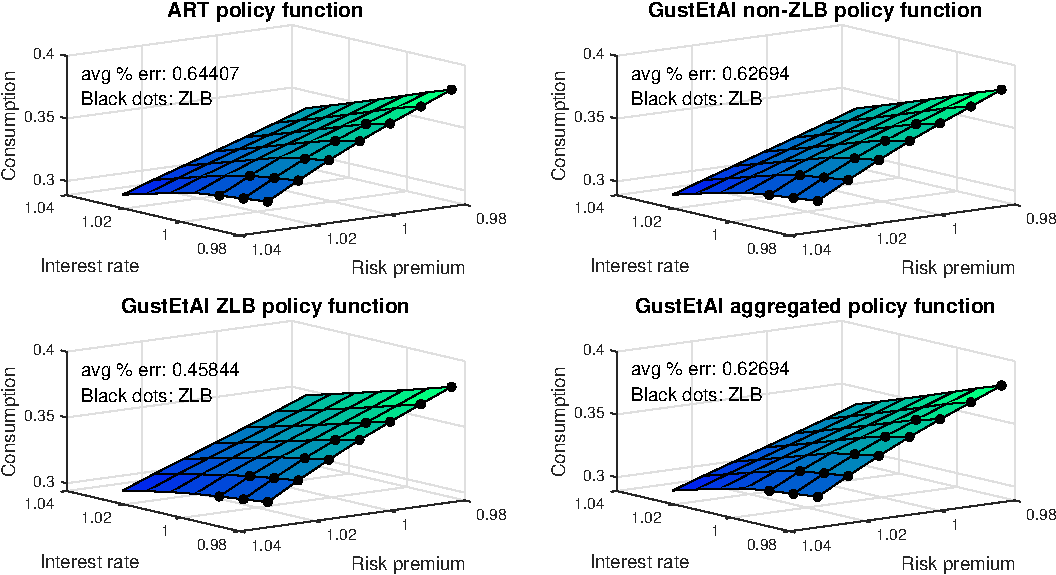
\includegraphics[width=10cm,scale=.3]{../Paper/pfs3D.pdf}
  \caption{Consumption policy function for model without capital}    
  \label{Fig:1}
  \end{figure}
\end{frame}

%===================================================================================
\begin{frame}\frametitle{Smoothness Measures}
\begin{table}[H]
  \centering
\captionsetup{justification=centering}
  \hypertarget{Table 3}
  \scriptsize
    \setlength{\tabcolsep}{4pt}      
  \begin{tabular}{l c c c c}
    \hline
    & \multicolumn{2}{c}{Model without capital} & \multicolumn{2}{c}{Model with capital} \\
    & Mean \% Error & RMSE & Mean \% Error & RMSE\\
    \hline
    ART policy & 0.64407\% &0.0027327 $c$  units & 0.271154\% & 0.0039806 $l$ units \\    
  GHLS policy & 0.62694\% & 0.0026704 $c$ units & 0.578098\% & 0.0080785 $l$ units \\
  \hline
\end{tabular}
  \caption{Smoothness measures for labor policy functions ($c$ for model with capital and $n$ for model with capital). GHLS combined policy functions are reported.}
\end{table} 
 \begin{itemize}\setlength{\itemsep}{8pt}
\item <1-|handout:1>RMSE (root mean square error)
\item <2-|handout:1>Mean percent error from linear policy functions
\item  <3-|handout:1>GHLS smoother for model without capital; ART smoother for model with capital
\end{itemize}
\end{frame}
%===================================================================================

\begin{frame}\frametitle{Euler Equation Errors: Model Without Capital}
% Distribution of the absolute value of the Euler equation errors in base 10 logarithms:
\begin{figure}[H]
    \centering
\captionsetup{justification=centering}
    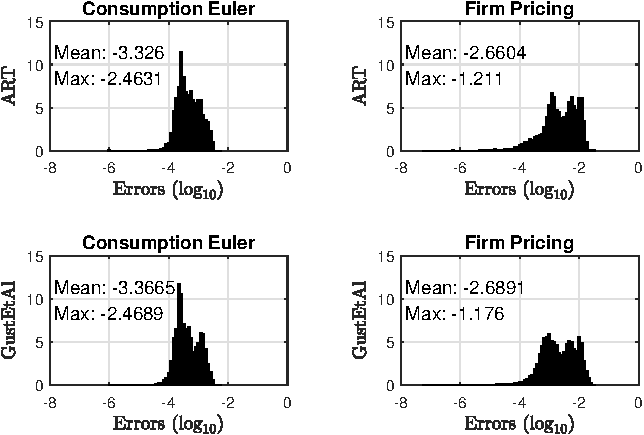
\includegraphics[width=9cm,scale=.74]{../Paper/eeerrors.pdf}
  \caption{Euler equation errors for model without capital}    
  \end{figure}
\end{frame}

%===================================================================================
\begin{frame}\frametitle{Policy Functions: Model with Capital} %black dots: ZLB, GHLS labor policy function is computed at and away from the ZLB and conmied later
\begin{figure}[H]
\hypertarget{Figure 1}  
    \centering
\captionsetup{justification=centering}
    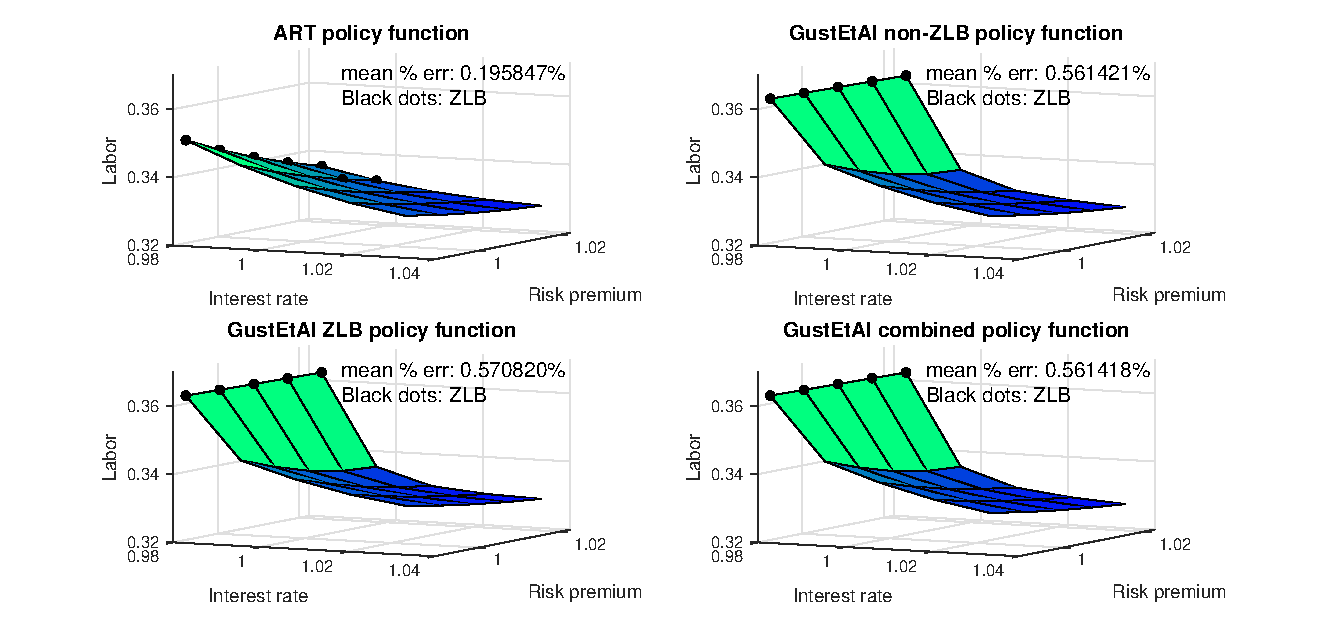
\includegraphics[width=10cm,scale=.3]{../Paper/pfs3DCAP.pdf}
  \caption{Labor policy function for model with capital}    
  \label{Fig:1}
  \end{figure}
\end{frame}
%===================================================================================

\begin{frame}\frametitle{Euler Equation Errors: Model With Capital}
 %Distribution of the absolute value of the Euler equation errors in base 10 logarithms:
\begin{figure}[H]
    \centering
\captionsetup{justification=centering}
    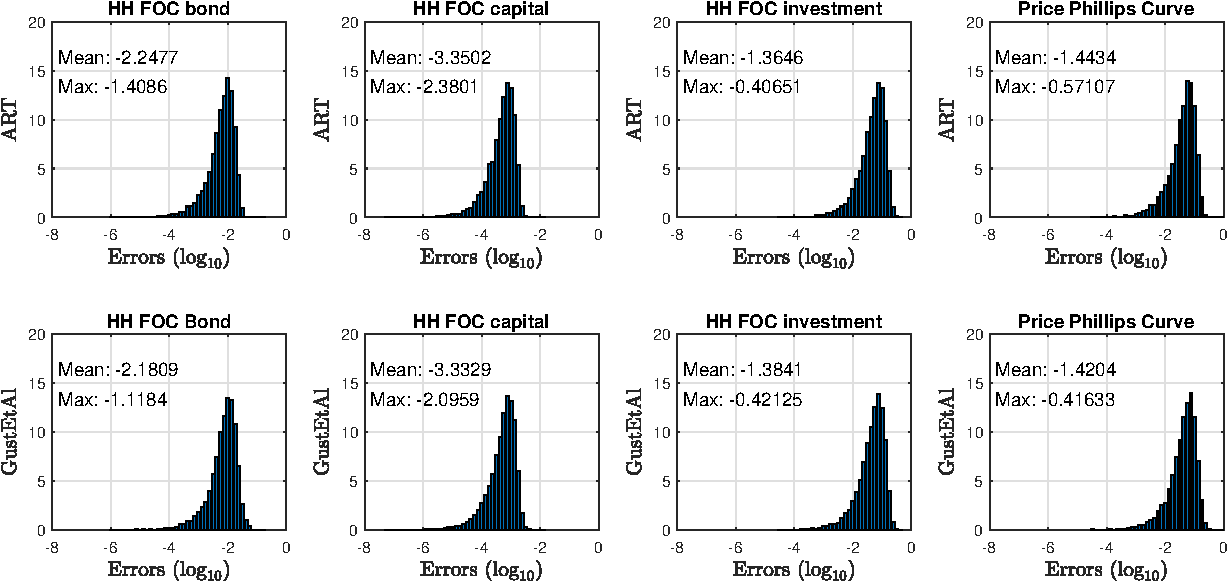
\includegraphics[width=10cm,scale=.8]{../Paper/eeerrorsCAP.pdf}
  \caption{Euler equation errors for model with capital}    
  \end{figure}
\end{frame}%Unlike the model with capital, GHLS performs better. 
%===================================================================================
\begin{frame}\frametitle{Conclusion}
\begin{itemize}\setlength{\itemsep}{8pt}
\item <1-|handout:1>During the Great Recession, policy rates hit zero, calling into question traditional solution methods
\item <2-|handout:1>There is a literature in solving nonlinear models, but not much work comparing nonlinear solution methods
\item <3-|handout:1>This paper discusses the impact of regime-indexing the policy functions on a nonlinear solution algorithm
\begin{enumerate}\setlength{\itemsep}{4pt}
\item Example of directly approximating the policy functions from Atkinson et al.\ (2019)
\item Example of for regime-indexing the policy functions from Gust et al.\ (2017). They claim that regime-indexed policy functions are smoother and easier to approximate
\end{enumerate}

\end{itemize}
\end{frame}

%===============================================================================================================
\begin{frame}\frametitle{Conclusion}
\begin{itemize}\setlength{\itemsep}{10pt}
\item <1-|handout:1>Key takeaways:
\begin{itemize}\setlength{\itemsep}{4pt}
\item In the model without capital, regime-indexed policy functions were smoother and solution algorithm was faster
\item In model with capital,  the regime-indexed policy functions were more nonlinear and solution algorithm was slower
\end{itemize}
\item <2-|handout:1>Extensions:
\begin{itemize}\setlength{\itemsep}{4pt}
\item Solve the GHLS solution method using Smolyak discretization methods and Chebyshev polynomials 
\item This would be expected to speed up the solution algorithm, but may lead to a less accurate solution
\end{itemize}
\end{itemize}
\end{frame}


\end{document}
